\documentclass[conference,a4paper]{IEEEtran}
\IEEEoverridecommandlockouts
 
\usepackage[indonesian]{babel}
\usepackage[utf8]{inputenc}
\usepackage[T1]{fontenc}
\usepackage{cite}
\usepackage{amsmath,amssymb}
\usepackage{graphicx}
\usepackage{booktabs}
\usepackage{siunitx}
\usepackage{xcolor}
\usepackage[hidelinks]{hyperref}
\graphicspath{{gambar/}}
 
% Penanda isian yang belum lengkap (hapus pemakaiannya di versi akhir)
\newcommand{\isi}[1]{\colorbox{yellow}{\textbf{[#1]}}}
 
% Pengaturan tabel agar muat satu kolom
\newcommand{\tabkecil}{\scriptsize\setlength{\tabcolsep}{2.5pt}}
 
\begin{document}
 
\title{Studi Ablasi RNN, LSTM, dan GRU dibandingkan ANN untuk Prediksi Trafik Seluler Kota Milan}
 
\author{
\IEEEauthorblockN{Alfita Eryani Nugroho}
\IEEEauthorblockA{NIM 124400002\\Teknik Telekomunikasi, ITERA\\alfita.124400002@student.itera.ac.id}
\and
\IEEEauthorblockN{Octavia Sesilia Malau}
\IEEEauthorblockA{NIM 124400038\\Teknik Telekomunikasi, ITERA\\octavia.124400038@student.itera.ac.id}
\and
\IEEEauthorblockN{Fitria Oktavianti}
\IEEEauthorblockA{NIM 124400058\\Teknik Telekomunikasi, ITERA\\fitria.124400058@student.itera.ac.id}
}
 
\maketitle
 
\begin{abstract}
Operator seluler perlu meramal trafik internet per jam agar kapasitas sel dapat diatur lebih awal. Studi ini membandingkan ANN dengan RNN, LSTM, dan GRU pada data Telecom Italia untuk kotak Duomo (5060) dan lokasi kelompok, Universita Bocconi (4460). Kami melakukan studi ablasi dengan mengubah satu faktor setiap kali, yaitu panjang jendela, ukuran hidden, jumlah lapisan, \textit{learning rate}, kelompok fitur, \textit{batch size}, \textit{dropout}, dan fungsi loss, masing-masing dengan 3 seed. Pada konfigurasi acuan, RNN terbaik dengan test MAE $229{,}6 \pm 5{,}1$, disusul GRU, LSTM, dan ANN ($309{,}9 \pm 5{,}9$). Setelah penyetelan, GRU terbaik dengan test MAE $221{,}9 \pm 14{,}3$, turun 6,5\,\% dari acuan dan 52,5\,\% lebih rendah daripada baseline naif terbaik, tetapi selisihnya dengan RNN ($226{,}3 \pm 4{,}9$) lebih kecil daripada simpangan baku. \textit{Learning rate} adalah faktor paling berpengaruh, sedangkan jendela panjang pada ANN, lapisan tambahan, dan \textit{dropout} tinggi merugikan. Di Bocconi urutan model berubah dan semua model kalah dari baseline naif nilai terakhir karena trafik turun menjelang Natal. Model rekuren ringan lebih andal daripada ANN, tetapi hasilnya bergantung pada pola trafik lokasi.
\end{abstract}
 
\begin{IEEEkeywords}
prediksi trafik seluler, RNN, LSTM, GRU, studi ablasi
\end{IEEEkeywords}
 
% ---------------------------------------------------------------------
\section{Pendahuluan}
Operator seluler perlu meramal trafik tiap sel agar kapasitas jaringan dapat diatur sebelum terjadi kemacetan dan agar energi tidak terbuang saat trafik sepi. Trafik per jam punya pola harian dan mingguan, sehingga model yang membaca urutan waktu, yaitu RNN, LSTM \cite{hochreiter1997lstm}, dan GRU \cite{cho2014gru}, diharapkan lebih baik daripada ANN yang memperlakukan jendela waktu sebagai deretan angka biasa. Namun, hasil tiap model sangat bergantung pada pengaturan \textit{hyperparameter}. Studi ablasi mengubah satu faktor setiap kali dan menjaga faktor lain tetap, sehingga pengaruh tiap faktor dapat dilihat dengan jelas. Kontribusi laporan ini:
\begin{itemize}
  \item membandingkan ANN, RNN, LSTM, dan GRU di kotak Duomo dengan baseline naif dan konfigurasi acuan;
  \item mengukur pengaruh lima faktor wajib dan tiga faktor pilihan dengan 3 seed;
  \item menguji konfigurasi terbaik di lokasi kelompok (Universita Bocconi) untuk melihat apakah hasilnya berlaku umum.
\end{itemize}
 
% ---------------------------------------------------------------------
\section{Data dan Metode}
 
\subsection{Dataset}
Kami memakai Telecom Italia Big Data Challenge \cite{barlacchi2015milan} versi per jam dari \cite{zhang2021fedda}. Data berisi aktivitas jaringan seluler per kotak di Milan dengan resolusi 1 jam dan tiga fitur: \textit{net} (aktivitas internet), \textit{call}, dan \textit{sms}. Periode yang dipakai adalah 4 November--29 Desember 2013 (8 minggu). Target prediksi adalah aktivitas internet (\textit{net}) satu jam ke depan. Eksperimen utama memakai kotak Duomo (5060). Lokasi kelompok kami untuk uji generalisasi adalah Universita Bocconi (kode 2, kotak 4460). Gambar~\ref{fig:peta} menunjukkan posisi 10 lokasi tugas di peta Milan, dan pola harian kedua lokasi dibandingkan pada Bagian~\ref{sec:generalisasi}: Duomo stabil, sedangkan trafik Bocconi turun tajam menjelang Natal.
 
\begin{figure}[t]
  \centering
  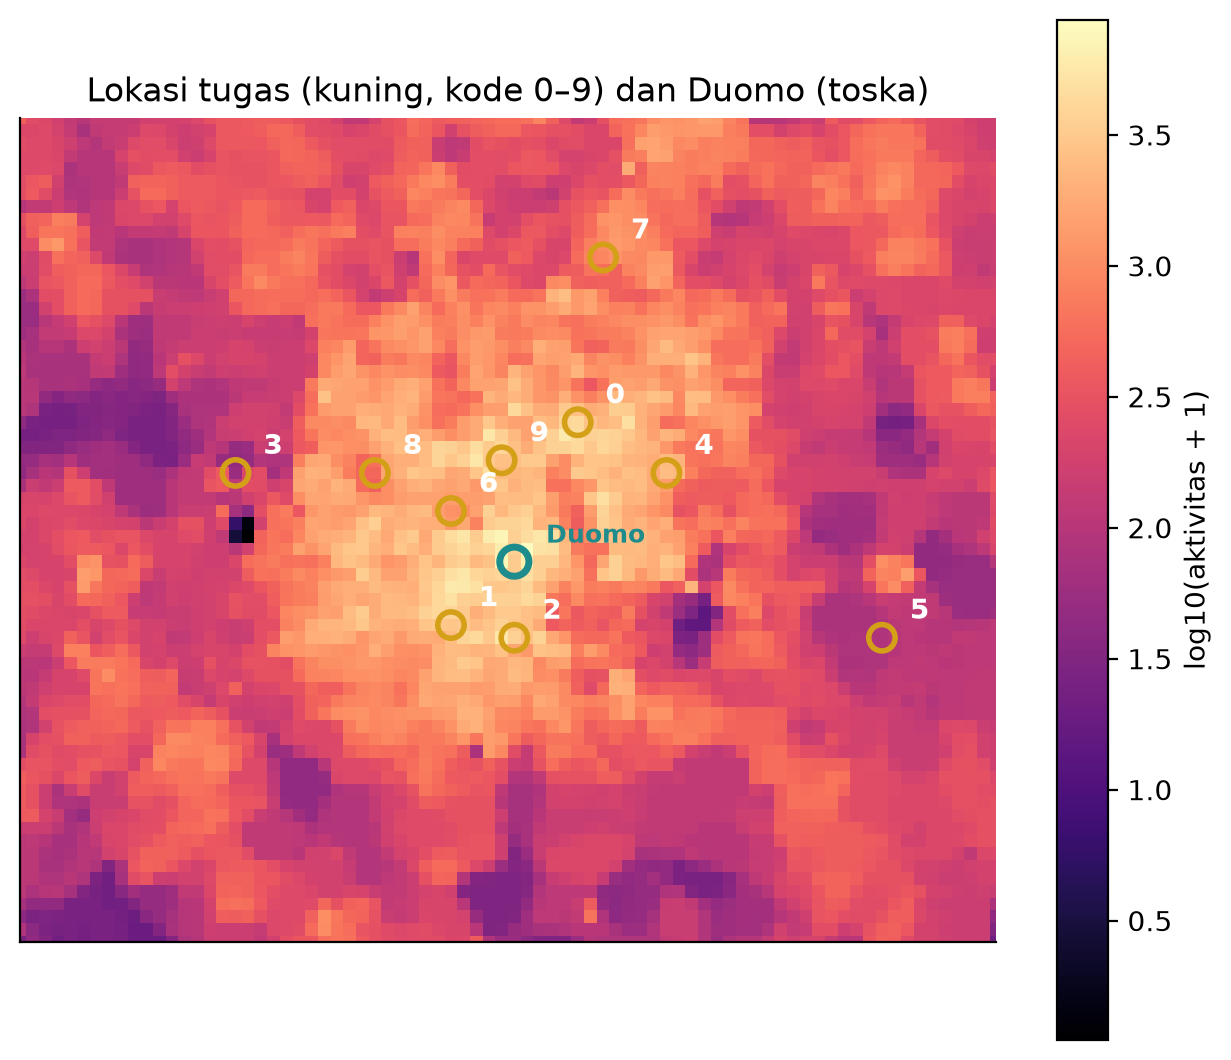
\includegraphics[width=0.85\linewidth]{peta_lokasi_tugas.png}
  \caption{Rata-rata aktivitas internet per kotak di Milan. Lingkaran kuning: lokasi tugas (kode 0--9); lingkaran toska: Duomo.}
  \label{fig:peta}
\end{figure}
 
\subsection{Pembagian Data dan Praproses}
Data dibagi berdasarkan waktu: \textit{train} 11 Nov--8 Des (4 minggu, 672 sampel), \textit{val} 9--15 Des, \textit{test} 16--22 Des, dan Natal 23--29 Des. Minggu pertama (4--10 Nov) hanya menjadi konteks jendela. Fitur (7 fitur: \textit{net}, \textit{call}, \textit{sms}, jam sin/cos, hari sin/cos) distandarisasi dengan statistik data sebelum minggu validasi, lalu dipotong menjadi jendela (\textit{windowing}) sepanjang $W$ jam untuk meramal 1 jam berikutnya. Data deret waktu tidak boleh diacak karena nilai sekarang bergantung pada nilai sebelumnya. Jika diacak, model ikut melihat data masa depan saat latihan (kebocoran data), sehingga hasil ujinya terlihat lebih bagus daripada kondisi nyata.
 
\subsection{Model dan Konfigurasi Acuan}
ANN meratakan jendela $[W, \text{fitur}]$ menjadi satu vektor, lalu melewatkannya ke lapisan tersembunyi (ReLU) dan lapisan output. RNN, LSTM, dan GRU membaca jendela jam demi jam sambil menyimpan \textit{hidden state}; keluaran \textit{hidden state} jam terakhir masuk ke lapisan output. RNN biasa mudah kehilangan informasi yang jauh. LSTM \cite{hochreiter1997lstm} dan GRU \cite{cho2014gru} memakai gerbang untuk memilih informasi yang disimpan, dan GRU lebih ringkas daripada LSTM. Analoginya, ANN seperti membaca seluruh catatan 24 jam sekaligus sebagai satu lembar angka, sedangkan RNN, LSTM, dan GRU seperti membaca catatan itu jam demi jam sambil membawa ringkasan di kepala; gerbang pada LSTM dan GRU berfungsi seperti keputusan mana yang dicatat dan mana yang dibuang. \textit{Dropout} dipasang setelah tiap lapisan tersembunyi ANN, di antara lapisan rekuren, dan sebelum lapisan output. Ukuran \textit{hidden} dipilih agar parameter model rekuren sekitar 5,5 ribu (Tabel~\ref{tab:acuan}).
 
\begin{table}[t]
  \centering
  \caption{Konfigurasi acuan}
  \label{tab:acuan}
  \tabkecil
  \begin{tabular}{@{}ll@{}}
    \toprule
    Hyperparameter & Nilai acuan \\
    \midrule
    Lokasi & Duomo (kotak 5060) \\
    Panjang jendela $W$ & 24 jam \\
    Horizon & 1 jam \\
    Ukuran hidden & ANN 32, RNN 68, LSTM 33, GRU 38 \\
    Jumlah lapisan & ANN 2, rekuren 1 \\
    Jumlah parameter & ANN 6.497, RNN 5.305, \\
     & LSTM 5.578, GRU 5.397 \\
    Fitur & net, call, sms, jam, hari (7) \\
    Optimizer, \textit{learning rate} & Adam, $10^{-3}$ \\
    \textit{Batch size} & 64 \\
    \textit{Dropout} & 0 \\
    Fungsi loss & MSE \\
    \textit{Early stopping} & \textit{patience} 30, maks.\ 300 epoch \\
    \bottomrule
  \end{tabular}
\end{table}
 
\subsection{Protokol Ablasi dan Evaluasi}
Satu faktor diubah setiap kali, faktor lain tetap pada acuan. Faktor wajib: A1 panjang jendela $W \in \{6, 12, 24, 48, 168\}$ jam; A2 ukuran \textit{hidden} $\in \{16, 32, 64, 128\}$; A3 jumlah lapisan $\in \{1, 2, 3\}$; A4 \textit{learning rate} $\in \{10^{-4}, 10^{-3}, 10^{-2}\}$; A5 kelompok fitur $\in$ \{net, net+call+sms, net+waktu, semua\}. Faktor pilihan: B1 \textit{batch size} $\in \{16, 64, 256\}$; B2 \textit{dropout} $\in \{0; 0{,}2; 0{,}5\}$; B4 fungsi loss $\in$ \{MSE, MAE, Huber\}. Hipotesis awal faktor B ada di Bagian~\ref{sec:pilihan}. Setiap konfigurasi dilatih dengan 3 \textit{seed} dan dilaporkan sebagai rata-rata $\pm$ simpangan baku (std). Metrik utama adalah MAE pada skala asli; MAPE dilaporkan untuk konfigurasi terbaik. Konfigurasi terbaik dipilih dengan val MAE rata-rata, bukan test. Perangkat: 13th Gen Intel Core dan Jupyter Notebook; total waktu training: 182,3 menit.
 
% ---------------------------------------------------------------------
\section{Hasil}
 
\subsection{Baseline Naif dan Acuan}
Tabel~\ref{tab:acuanhasil} memuat tiga baseline naif (meniru nilai jam terakhir, jam yang sama kemarin, dan jam yang sama minggu lalu) dan hasil konfigurasi acuan. Pada minggu test, baseline terbaik adalah ``minggu lalu'' (467,6) karena trafik berulang tiap minggu. Pada minggu Natal pola mingguan rusak karena libur, sehingga ``minggu lalu'' memburuk menjadi 1.426,2 dan ``nilai terakhir'' menjadi yang terbaik (431,2). Semua model acuan mengalahkan baseline terbaik pada minggu test: RNN 229,6 (sekitar 51\,\% lebih rendah), GRU 237,2, LSTM 273,6, dan ANN 309,9. LSTM paling tidak stabil antar seed ($\pm 25{,}4$). Pada minggu Natal hanya RNN (421,2) yang mengalahkan baseline 431,2, sedangkan GRU (468,2), LSTM (586,0), dan ANN (680,1) lebih buruk.
 
\begin{table}[t]
  \centering
  \caption{Baseline naif dan konfigurasi acuan di Duomo (MAE)}
  \label{tab:acuanhasil}
  \tabkecil
  \begin{tabular}{@{}lccc@{}}
    \toprule
    Model & Val & Test & Natal \\
    \midrule
    \multicolumn{4}{@{}l}{\textit{Baseline naif (horizon 1 jam)}} \\
    Nilai terakhir & 662,6 & 600,9 & 431,2 \\
    Kemarin & 595,3 & 552,2 & 921,5 \\
    Minggu lalu & 492,8 & \textbf{467,6} & 1.426,2 \\
    \midrule
    \multicolumn{4}{@{}l}{\textit{Konfigurasi acuan (rata-rata $\pm$ std, 3 seed)}} \\
    ANN & $248{,}9 \pm 8{,}9$ & $309{,}9 \pm 5{,}9$ & $680{,}1 \pm 52{,}0$ \\
    RNN & $206{,}1 \pm 7{,}4$ & $\mathbf{229{,}6 \pm 5{,}1}$ & $\mathbf{421{,}2 \pm 2{,}4}$ \\
    LSTM & $230{,}5 \pm 12{,}2$ & $273{,}6 \pm 25{,}4$ & $586{,}0 \pm 56{,}8$ \\
    GRU & $207{,}5 \pm 3{,}8$ & $237{,}2 \pm 9{,}3$ & $468{,}2 \pm 21{,}8$ \\
    \bottomrule
  \end{tabular}
\end{table}
 
\subsection{Ablasi Wajib}
Hasil lima faktor wajib ada di Gambar~\ref{fig:a1}--\ref{fig:a5} dan Tabel~\ref{tab:a}. Angka tebal pada Tabel~\ref{tab:a} adalah test MAE terkecil untuk tiap model dalam satu faktor.
 
\textbf{A1. Panjang jendela (Gambar~\ref{fig:a1}).} Jendela lebih panjang tidak selalu lebih baik. Pada ANN, test MAE naik dari 271,1 ($W=6$) menjadi 402,0 ($W=168$) karena jumlah parameternya membengkak dari 2.465 menjadi 38.753, padahal data latih hanya 672 sampel sehingga ANN mudah \textit{overfit}. Model rekuren hampir tidak terpengaruh karena jumlah parameternya tetap: RNN 224,5--233,5, GRU 237,1--249,8, dan LSTM 273,6--304,4. RNN paling stabil terhadap $W$. Analoginya seperti menebak cuaca besok: melihat 6 jam terakhir mungkin kurang, tetapi menghafal 168 jam sekaligus membuat ANN ``kebanyakan catatan'' untuk dihafal dari hanya 672 contoh, sedangkan model rekuren cukup memakai aturan baca yang sama untuk tiap jam.
 
\textbf{A2. Ukuran hidden (Gambar~\ref{fig:a2}).} Model yang lebih besar tidak selalu lebih baik. GRU dan LSTM membaik saat \textit{hidden} membesar: test MAE GRU turun dari 246,9 (\textit{hidden} 16) ke 220,3 (\textit{hidden} 128), dan LSTM dari 295,3 ke 245,6. RNN sudah baik sejak \textit{hidden} 32 (245,2) dan hanya membaik tipis menjadi 234,6 dengan std besar ($\pm 18{,}6$), sedangkan ANN hampir datar (304,9--315,3). Pada \textit{hidden} 128, LSTM punya 70.273 parameter, hampir 4 kali RNN (17.665), tetapi hasilnya tidak jauh berbeda (245,6 vs 234,6). Ukuran \textit{hidden} dapat dibayangkan sebagai besar meja kerja: meja yang lebih luas memudahkan LSTM dan GRU yang membawa banyak ``catatan'' (gerbang), sementara RNN yang catatannya sedikit sudah cukup dengan meja sedang.
 
\begin{figure}[t]
  \centering
  
\includegraphics[width=\linewidth]{A1_W.png}
  \caption{Pengaruh panjang jendela $W$ terhadap val MAE (kiri) dan test MAE (kanan). Garis: rata-rata 3 seed; area berwarna: sebaran antar seed.}
  \label{fig:a1}
\end{figure}
 
\begin{figure}[t]
  \centering
  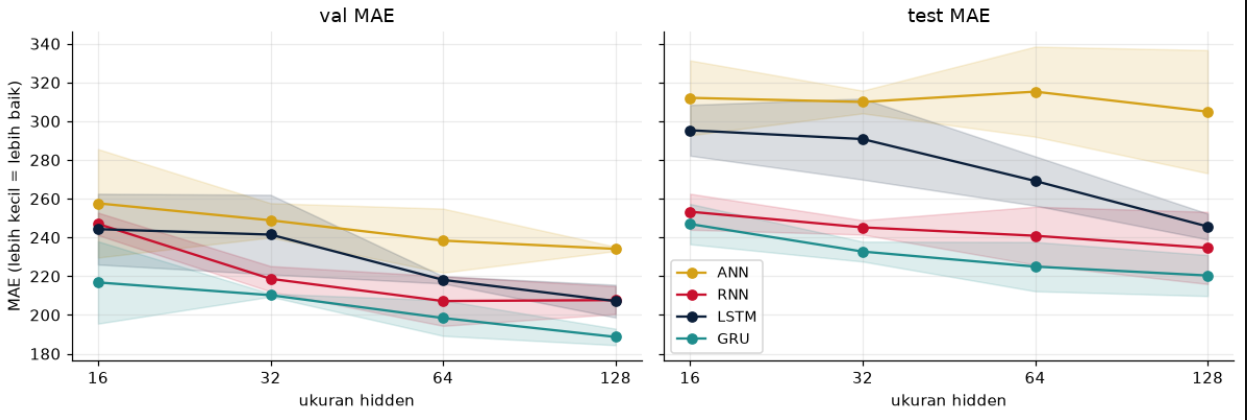
\includegraphics[width=\linewidth]{A2_hidden.png}
  \caption{Pengaruh ukuran \textit{hidden} terhadap val MAE (kiri) dan test MAE (kanan).}
  \label{fig:a2}
\end{figure}
 
\textbf{A3. Jumlah lapisan (Gambar~\ref{fig:a3}).} Menumpuk lapisan tidak membantu. RNN dan GRU nyaris sama pada 1--2 lapisan (RNN 229,6 $\to$ 228,4; GRU 237,2 $\to$ 239,2) dan memburuk pada 3 lapisan (245,5 dan 264,2). LSTM paling sensitif: 273,6 $\to$ 308,9 $\to$ 412,6, dan val MAE-nya ikut naik dari 230,5 menjadi 338,9, jadi LSTM bertingkat sulit dilatih dengan 672 sampel. Model yang lebih dalam juga cenderung berhenti lebih awal (epoch rata-rata RNN turun dari 163,7 menjadi 96,0), tanda lebih cepat \textit{overfit}. ANN relatif stabil (299,8--311,6). Analoginya seperti permainan pesan berantai: makin banyak orang di tengah, makin besar kemungkinan pesan berubah, apalagi bila ``pelatihnya'' hanya punya 672 contoh.
 
\textbf{A4. \textit{Learning rate} (Gambar~\ref{fig:a4}).} Ini faktor paling berpengaruh. Pada $10^{-4}$ semua model berhenti di batas 300 epoch sebelum konvergen dan hasilnya buruk (test MAE RNN 287,9; GRU 356,3; LSTM 373,5; ANN 339,5). Pada $10^{-2}$ training jauh lebih cepat (62--68 epoch dibanding 106--194 pada acuan), dan LSTM serta GRU justru terbaik ($225{,}8 \pm 4{,}2$ dan $215{,}7 \pm 10{,}9$). RNN sedikit memburuk (244,4), sedangkan ANN tidak membaik dan std-nya sangat besar ($\pm 53{,}2$), tanda training kurang stabil. \textit{Learning rate} seperti ukuran langkah saat menuruni bukit berkabut: langkah terlalu kecil ($10^{-4}$) tidak sampai ke lembah dalam 300 epoch, langkah terlalu besar bisa melompati lembah, dan langkah menengah paling aman.
 
\begin{figure}[t]
  \centering
  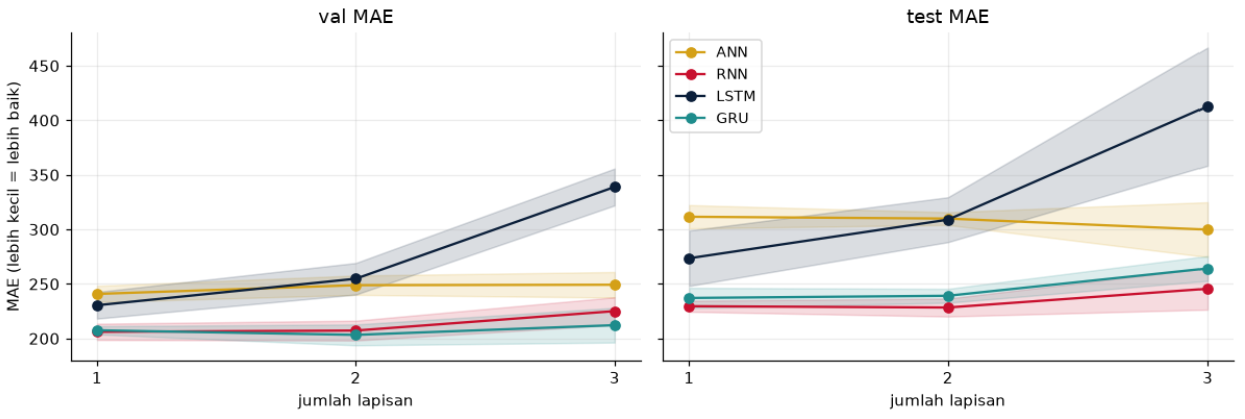
\includegraphics[width=\linewidth]{A3_layers.png}
  \caption{Pengaruh jumlah lapisan terhadap val MAE (kiri) dan test MAE (kanan).}
  \label{fig:a3}
\end{figure}
 
\begin{figure}[t]
  \centering
  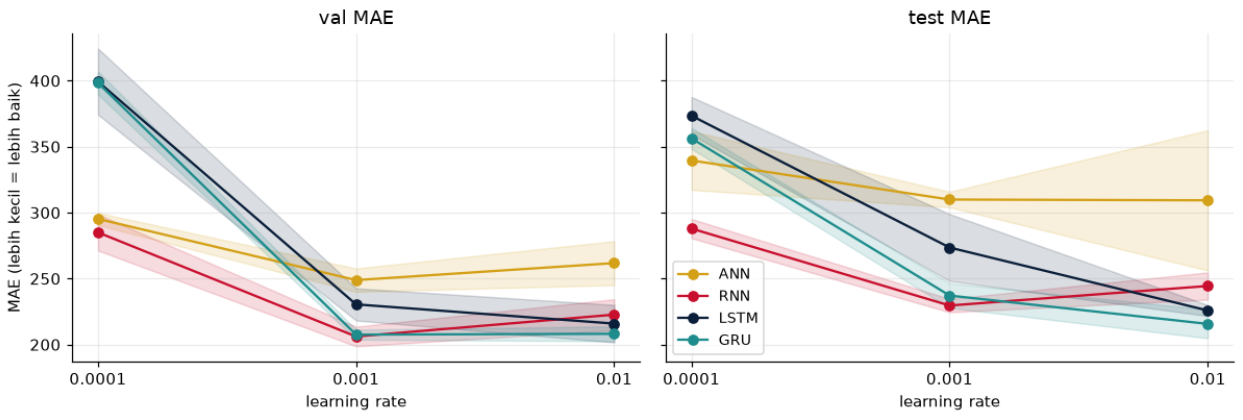
\includegraphics[width=\linewidth]{A4_lr.png}
  \caption{Pengaruh \textit{learning rate} terhadap val MAE (kiri) dan test MAE (kanan).}
  \label{fig:a4}
\end{figure}
 
\textbf{A5. Kelompok fitur (Gambar~\ref{fig:a5}).} Fitur tambahan tidak selalu membantu. Trafik telepon dan SMS paling berguna bagi RNN dan LSTM: net+call+sms memberi test MAE terbaik (RNN $227{,}6 \pm 2{,}2$; LSTM 262,7). Dibanding itu, fitur jam dan hari tidak memberi tambahan (RNN 244,9; LSTM 292,6), kemungkinan karena model rekuren sudah membaca pola harian dari urutan jendela. GRU mendapat manfaat dari kedua jenis fitur (270,5 dengan \textit{net} saja menjadi 237,2 dengan semua fitur). ANN justru terbaik hanya dengan \textit{net} ($271{,}7 \pm 13{,}9$) dan memburuk bila fitur ditambah (309,9), kemungkinan karena input yang lebih banyak membuat ANN lebih mudah \textit{overfit}. Analoginya, fitur adalah petunjuk bagi penebak: model rekuren bisa memilah banyak petunjuk, tetapi ANN yang menerima terlalu banyak petunjuk sekaligus mudah bingung dan menghafal.
 
\begin{table}[t]
  \centering
  \caption{Pengaruh faktor A1--A5 terhadap test MAE (rata-rata $\pm$ std, 3 seed)}
  \label{tab:a}
  \tabkecil
  \begin{tabular}{@{}lcccc@{}}
    \toprule
    Nilai & ANN & RNN & LSTM & GRU \\
    \midrule
    \multicolumn{5}{@{}l}{\textit{A1. Panjang jendela $W$ (jam)}} \\
    6   & $\mathbf{271{,}1 \pm 13{,}9}$ & $228{,}6 \pm 5{,}4$ & $276{,}3 \pm 14{,}7$ & $249{,}8 \pm 1{,}4$ \\
    12  & $310{,}8 \pm 14{,}8$ & $233{,}2 \pm 11{,}2$ & $302{,}7 \pm 17{,}4$ & $246{,}1 \pm 13{,}5$ \\
    24  & $309{,}9 \pm 5{,}9$ & $229{,}6 \pm 5{,}1$ & $\mathbf{273{,}6 \pm 25{,}4}$ & $237{,}2 \pm 9{,}3$ \\
    48  & $333{,}1 \pm 20{,}3$ & $\mathbf{224{,}5 \pm 11{,}7}$ & $304{,}4 \pm 27{,}1$ & $\mathbf{237{,}1 \pm 10{,}6}$ \\
    168 & $402{,}0 \pm 12{,}5$ & $233{,}5 \pm 4{,}8$ & $292{,}8 \pm 20{,}0$ & $237{,}2 \pm 10{,}6$ \\
    \midrule
    \multicolumn{5}{@{}l}{\textit{A2. Ukuran hidden}} \\
    16  & $312{,}1 \pm 19{,}3$ & $253{,}3 \pm 9{,}3$ & $295{,}3 \pm 13{,}1$ & $246{,}9 \pm 10{,}4$ \\
    32  & $309{,}9 \pm 5{,}9$ & $245{,}2 \pm 3{,}7$ & $290{,}8 \pm 20{,}9$ & $232{,}7 \pm 5{,}1$ \\
    64  & $315{,}3 \pm 23{,}2$ & $240{,}9 \pm 15{,}0$ & $269{,}2 \pm 12{,}7$ & $225{,}0 \pm 12{,}7$ \\
    128 & $\mathbf{304{,}9 \pm 31{,}8}$ & $\mathbf{234{,}6 \pm 18{,}6}$ & $\mathbf{245{,}6 \pm 6{,}7}$ & $\mathbf{220{,}3 \pm 10{,}6}$ \\
    \midrule
    \multicolumn{5}{@{}l}{\textit{A3. Jumlah lapisan}} \\
    1 & $311{,}6 \pm 10{,}7$ & $229{,}6 \pm 5{,}1$ & $\mathbf{273{,}6 \pm 25{,}4}$ & $\mathbf{237{,}2 \pm 9{,}3}$ \\
    2 & $309{,}9 \pm 5{,}9$ & $\mathbf{228{,}4 \pm 8{,}2}$ & $308{,}9 \pm 20{,}6$ & $239{,}2 \pm 6{,}4$ \\
    3 & $\mathbf{299{,}8 \pm 25{,}1}$ & $245{,}5 \pm 19{,}1$ & $412{,}6 \pm 54{,}2$ & $264{,}2 \pm 11{,}4$ \\
    \midrule
    \multicolumn{5}{@{}l}{\textit{A4. \textit{Learning rate}}} \\
    $10^{-4}$ & $339{,}5 \pm 22{,}3$ & $287{,}9 \pm 7{,}3$ & $373{,}5 \pm 14{,}3$ & $356{,}3 \pm 7{,}9$ \\
    $10^{-3}$ & $309{,}9 \pm 5{,}9$ & $\mathbf{229{,}6 \pm 5{,}1}$ & $273{,}6 \pm 25{,}4$ & $237{,}2 \pm 9{,}3$ \\
    $10^{-2}$ & $\mathbf{309{,}4 \pm 53{,}2}$ & $244{,}4 \pm 10{,}3$ & $\mathbf{225{,}8 \pm 4{,}2}$ & $\mathbf{215{,}7 \pm 10{,}9}$ \\
    \midrule
    \multicolumn{5}{@{}l}{\textit{A5. Kelompok fitur}} \\
    net & $\mathbf{271{,}7 \pm 13{,}9}$ & $254{,}1 \pm 1{,}7$ & $284{,}1 \pm 19{,}3$ & $270{,}5 \pm 10{,}9$ \\
    net+call+sms & $315{,}9 \pm 12{,}2$ & $\mathbf{227{,}6 \pm 2{,}2}$ & $\mathbf{262{,}7 \pm 10{,}9}$ & $250{,}7 \pm 9{,}3$ \\
    net+waktu & $296{,}4 \pm 9{,}1$ & $244{,}9 \pm 22{,}1$ & $292{,}6 \pm 25{,}1$ & $239{,}7 \pm 25{,}4$ \\
    semua & $309{,}9 \pm 5{,}9$ & $229{,}6 \pm 5{,}1$ & $273{,}6 \pm 25{,}4$ & $\mathbf{237{,}2 \pm 9{,}3}$ \\
    \bottomrule
  \end{tabular}
\end{table}
 
\begin{figure}[t]
  \centering
  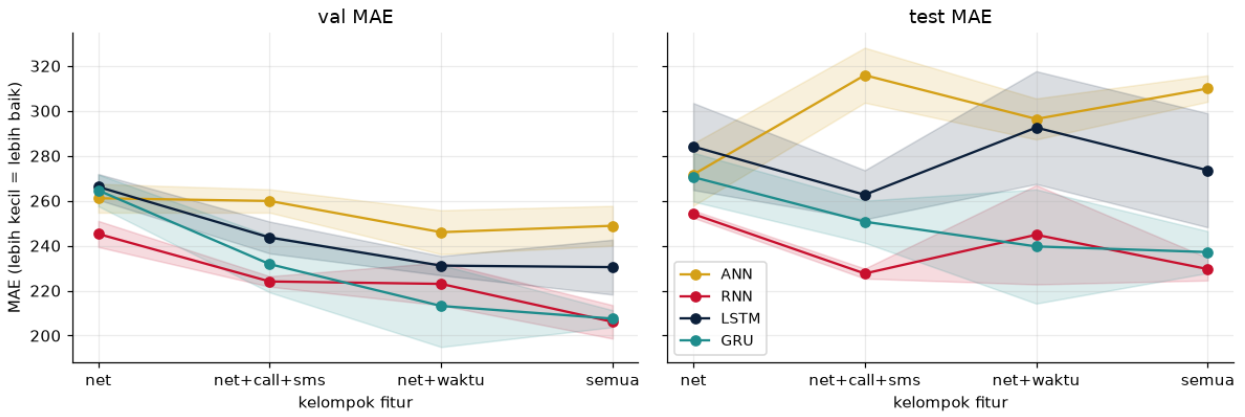
\includegraphics[width=\linewidth]{A5_fitur.png}
  \caption{Pengaruh kelompok fitur terhadap val MAE (kiri) dan test MAE (kanan).}
  \label{fig:a5}
\end{figure}
 
\subsection{Ablasi Pilihan}
\label{sec:pilihan}
Kami memilih tiga faktor tambahan: \textit{batch size}, \textit{dropout}, dan fungsi loss (Gambar~\ref{fig:b1}--\ref{fig:b4}, Tabel~\ref{tab:b}).
 
\textbf{B1. \textit{Batch size} (Gambar~\ref{fig:b1}).} \textit{Hipotesis:} batch kecil membuat pembaruan bobot lebih sering sehingga lebih akurat, tetapi lebih berisik. \textit{Hasil:} batch 16 sama atau lebih baik daripada 64, terutama pada LSTM (273,6 $\to$ 248,9), dan butuh epoch jauh lebih sedikit (79--112 vs 106--194). Batch 256 paling buruk pada semua model (ANN 320,1; RNN 258,9; LSTM 308,8; GRU 263,9), dan GRU menyentuh batas 300 epoch. Std test pada batch 16 sedikit lebih besar untuk keempat model. \textit{Hipotesis terbukti}, walau untuk RNN dan GRU selisih batch 16 dan 64 lebih kecil daripada std. Seperti guru yang mengoreksi latihan: memeriksa 16 soal lalu langsung memperbaiki cara belajar jauh lebih sering daripada menunggu 256 soal baru memperbaiki sekali.
 
\textbf{B2. \textit{Dropout} (Gambar~\ref{fig:b2}).} \textit{Hipotesis:} \textit{dropout} membantu karena data latih kecil dan rawan \textit{overfit}. \textit{Hasil:} \textit{dropout} tidak membantu. ANN memburuk paling jelas (309,9 $\to$ 330,1 $\to$ 411,6 pada \textit{dropout} 0 $\to$ 0,2 $\to$ 0,5), dan val MAE-nya ikut naik dari 248,9 menjadi 377,7. RNN memburuk menjadi sekitar 260 pada kedua nilai \textit{dropout}, LSTM berubah kecil (264,6--289,1), dan GRU hanya sedikit membaik pada 0,2 (225,0 vs 237,2) yang masih di dalam std ($\pm 12{,}8$). \textit{Hipotesis tidak terbukti:} model sudah kecil (sekitar 5 ribu parameter), sehingga \textit{dropout} kuat lebih mungkin menyebabkan \textit{underfit}, terlihat dari val MAE yang juga naik. \textit{Dropout} seperti belajar dengan menutup sebagian catatan secara acak; berguna bila catatan berlimpah, tetapi bila model sudah kecil, catatan yang ditutup justru membuatnya kekurangan bahan.
 
\textbf{B4. Fungsi loss (Gambar~\ref{fig:b4}).} \textit{Hipotesis:} loss MAE paling cocok untuk metrik MAE karena langsung meminimalkannya, sedangkan MSE lebih sensitif terhadap lonjakan trafik. \textit{Hasil:} loss MAE memberi test MAE terendah untuk keempat model, tetapi selisih besar hanya pada RNN (229,6 $\to$ $207{,}6 \pm 2{,}8$, turun 9,6\,\%). Pada ANN (297,2; selisih 12,7), LSTM (265,9; selisih 7,7), dan GRU (229,4; selisih 7,8), selisihnya sebanding dengan atau lebih kecil daripada std. Huber hampir sama dengan MSE. \textit{Hipotesis terbukti kuat pada RNN dan lemah pada model lain.} Catatan: val MAE RNN dengan loss MAE (212,5) lebih buruk daripada MSE (206,1), sehingga pemilihan lewat val tidak akan memilihnya. Analoginya, MSE seperti guru yang menghukum kesalahan besar jauh lebih berat, sedangkan MAE menghukum sebanding dengan besar kesalahan, sehingga lebih cocok bila nilai ujiannya juga dihitung dengan MAE.
 
\begin{table}[t]
  \centering
  \caption{Pengaruh faktor pilihan B1, B2, B4 terhadap test MAE (rata-rata $\pm$ std, 3 seed)}
  \label{tab:b}
  \tabkecil
  \begin{tabular}{@{}lcccc@{}}
    \toprule
    Nilai & ANN & RNN & LSTM & GRU \\
    \midrule
    \multicolumn{5}{@{}l}{\textit{B1. Batch size}} \\
    16  & $\mathbf{302{,}1 \pm 12{,}8}$ & $\mathbf{228{,}3 \pm 6{,}7}$ & $\mathbf{248{,}9 \pm 35{,}2}$ & $\mathbf{232{,}2 \pm 10{,}3}$ \\
    64  & $309{,}9 \pm 5{,}9$ & $229{,}6 \pm 5{,}1$ & $273{,}6 \pm 25{,}4$ & $237{,}2 \pm 9{,}3$ \\
    256 & $320{,}1 \pm 29{,}0$ & $258{,}9 \pm 32{,}5$ & $308{,}8 \pm 4{,}3$ & $263{,}9 \pm 3{,}7$ \\
    \midrule
    \multicolumn{5}{@{}l}{\textit{B2. Dropout}} \\
    0   & $\mathbf{309{,}9 \pm 5{,}9}$ & $\mathbf{229{,}6 \pm 5{,}1}$ & $273{,}6 \pm 25{,}4$ & $237{,}2 \pm 9{,}3$ \\
    0,2 & $330{,}1 \pm 47{,}0$ & $260{,}3 \pm 13{,}1$ & $\mathbf{264{,}6 \pm 16{,}6}$ & $\mathbf{225{,}0 \pm 12{,}8}$ \\
    0,5 & $411{,}6 \pm 8{,}0$ & $260{,}2 \pm 6{,}4$ & $289{,}1 \pm 10{,}3$ & $273{,}6 \pm 20{,}5$ \\
    \midrule
    \multicolumn{5}{@{}l}{\textit{B4. Fungsi loss}} \\
    MSE   & $309{,}9 \pm 5{,}9$ & $229{,}6 \pm 5{,}1$ & $273{,}6 \pm 25{,}4$ & $237{,}2 \pm 9{,}3$ \\
    MAE   & $\mathbf{297{,}2 \pm 10{,}9}$ & $\mathbf{207{,}6 \pm 2{,}8}$ & $\mathbf{265{,}9 \pm 17{,}8}$ & $\mathbf{229{,}4 \pm 16{,}5}$ \\
    Huber & $315{,}6 \pm 4{,}6$ & $225{,}3 \pm 3{,}0$ & $271{,}6 \pm 30{,}3$ & $236{,}5 \pm 7{,}7$ \\
    \bottomrule
  \end{tabular}
\end{table}
 
\begin{figure}[t]
  \centering
  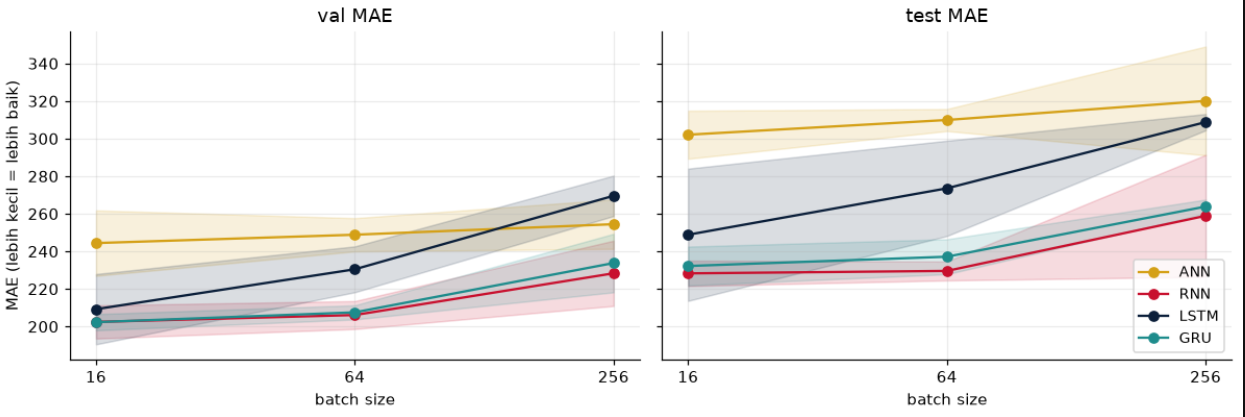
\includegraphics[width=\linewidth]{B1_batch.png}
  \caption{Pengaruh \textit{batch size} terhadap val MAE (kiri) dan test MAE (kanan).}
  \label{fig:b1}
\end{figure}
 
\begin{figure}[t]
  \centering
  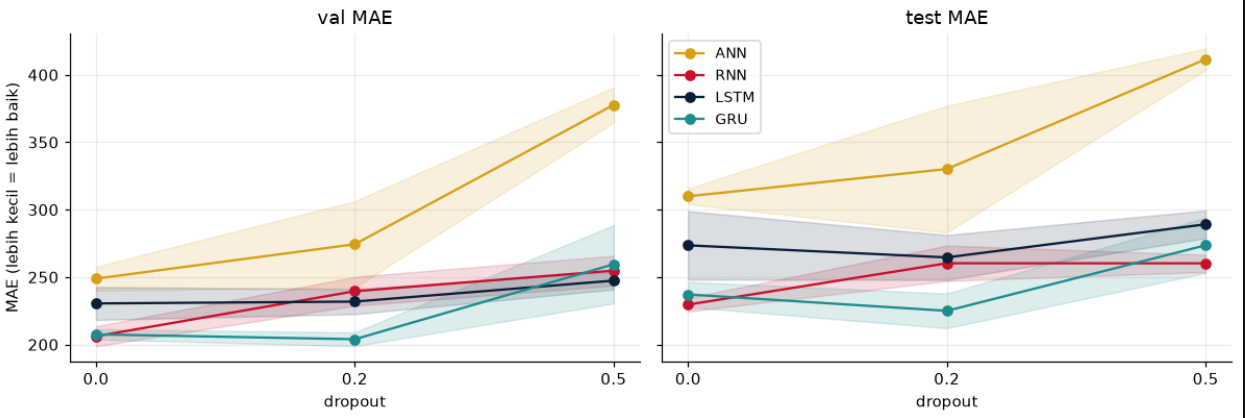
\includegraphics[width=\linewidth]{B2_dropout.png}
  \caption{Pengaruh \textit{dropout} terhadap val MAE (kiri) dan test MAE (kanan).}
  \label{fig:b2}
\end{figure}
 
\begin{figure}[t]
  \centering
  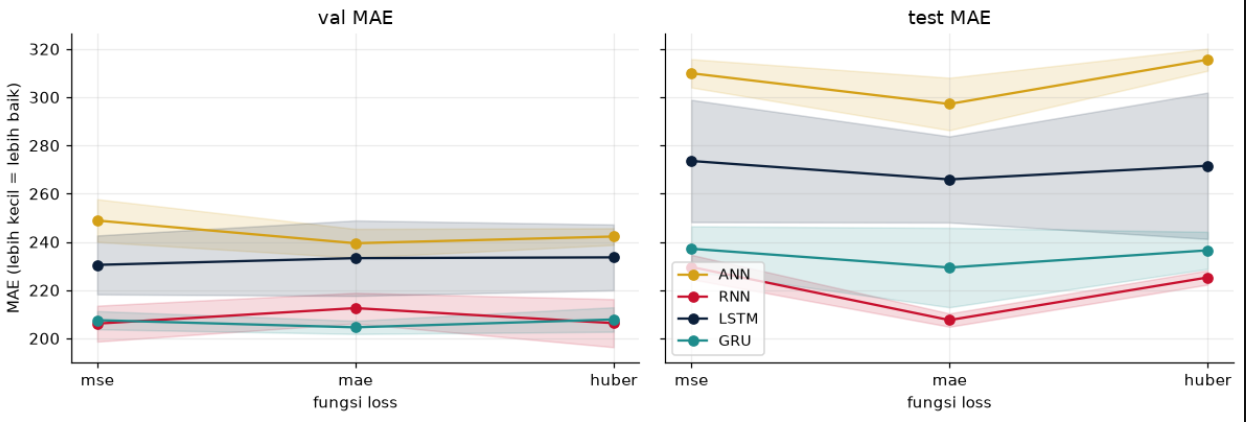
\includegraphics[width=\linewidth]{B4_loss.png}
  \caption{Pengaruh fungsi loss terhadap val MAE (kiri) dan test MAE (kanan).}
  \label{fig:b4}
\end{figure}
 
\subsection{Konfigurasi Terbaik}
Nilai terbaik tiap faktor digabung per model berdasarkan val MAE, lalu hasilnya diuji pada minggu test dan Natal (Tabel~\ref{tab:terbaik}, Gambar~\ref{fig:terbaik}). Konfigurasi terbaik: ANN ($W=6$, \textit{hidden} 128, 1 lapisan, fitur net+waktu, batch 16, loss MAE); RNN ($W=48$, batch 16); LSTM ($W=6$, \textit{hidden} 128, \textit{learning rate} $10^{-2}$, batch 16); GRU ($W=48$, \textit{hidden} 128, 2 lapisan, batch 16, \textit{dropout} 0,2, loss MAE); faktor yang tidak disebut memakai nilai acuan. Test MAE turun pada semua model: ANN 11,6\,\% (309,9 $\to$ 273,9), LSTM 9,9\,\% (273,6 $\to$ 246,6), GRU 6,5\,\% (237,2 $\to$ 221,9), dan RNN 1,4\,\% (229,6 $\to$ 226,3). Urutan akhirnya GRU, RNN, LSTM, ANN, tetapi selisih GRU dan RNN (4,4) jauh lebih kecil daripada std GRU ($\pm 14{,}3$), sehingga keduanya setara. Semua model berada jauh di bawah baseline naif terbaik (467,6); GRU terbaik 52,5\,\% lebih rendah. Ukuran model ikut berubah: GRU terbaik punya 151.809 parameter (28 kali acuan) dan LSTM 70.273 (12,6 kali), sedangkan ANN mengecil menjadi 4.097 dan RNN tetap. Pada minggu Natal hanya RNN terbaik ($385{,}4 \pm 13{,}8$) yang mengalahkan baseline nilai terakhir (431,2). Perhatikan juga bahwa val MAE RNN, LSTM, dan GRU pada konfigurasi gabungan sedikit lebih buruk daripada acuan (misalnya GRU 216,4 vs 207,5), artinya nilai terbaik per faktor belum tentu terbaik saat digabung. Ini seperti memilih bahan terbaik untuk tiap bumbu secara terpisah: setelah dicampur, rasanya belum tentu paling enak karena bahan saling memengaruhi.
 
\begin{table}[t]
  \centering
  \caption{Konfigurasi acuan dan terbaik di Duomo (rata-rata $\pm$ std, 3 seed)}
  \label{tab:terbaik}
  \tabkecil
  \setlength{\tabcolsep}{1.6pt}
  \resizebox{\columnwidth}{!}{%
\begin{tabular}{@{}llrcccc@{}}
    \toprule
    Model & Konf. & Param. & Val MAE & Test MAE & MAPE (\%) & Natal MAE \\
    \midrule
    ANN  & acuan   & 6.497   & $248{,}9 \pm 8{,}9$ & $309{,}9 \pm 5{,}9$ & $11{,}3 \pm 0{,}8$ & $680{,}1 \pm 52{,}0$ \\
         & terbaik & 4.097   & $218{,}4 \pm 10{,}8$ & $273{,}9 \pm 17{,}0$ & $9{,}3 \pm 0{,}8$ & $572{,}6 \pm 49{,}0$ \\
    RNN  & acuan   & 5.305   & $206{,}1 \pm 7{,}4$ & $229{,}6 \pm 5{,}1$ & $8{,}5 \pm 0{,}3$ & $421{,}2 \pm 2{,}4$ \\
         & terbaik & 5.305   & $209{,}5 \pm 3{,}2$ & $226{,}3 \pm 4{,}9$ & $8{,}2 \pm 0{,}7$ & $\mathbf{385{,}4 \pm 13{,}8}$ \\
    LSTM & acuan   & 5.578   & $230{,}5 \pm 12{,}2$ & $273{,}6 \pm 25{,}4$ & $9{,}1 \pm 1{,}0$ & $586{,}0 \pm 56{,}8$ \\
         & terbaik & 70.273  & $241{,}1 \pm 4{,}9$ & $246{,}6 \pm 12{,}0$ & $8{,}5 \pm 0{,}5$ & $462{,}7 \pm 5{,}2$ \\
    GRU  & acuan   & 5.397   & $207{,}5 \pm 3{,}8$ & $237{,}2 \pm 9{,}3$ & $8{,}0 \pm 0{,}7$ & $468{,}2 \pm 21{,}8$ \\
         & terbaik & 151.809 & $216{,}4 \pm 2{,}6$ & $\mathbf{221{,}9 \pm 14{,}3}$ & $\mathbf{7{,}1 \pm 0{,}7}$ & $454{,}8 \pm 18{,}1$ \\
    \bottomrule
  \end{tabular}}
\end{table}
 
\begin{figure}[t]
  \centering
  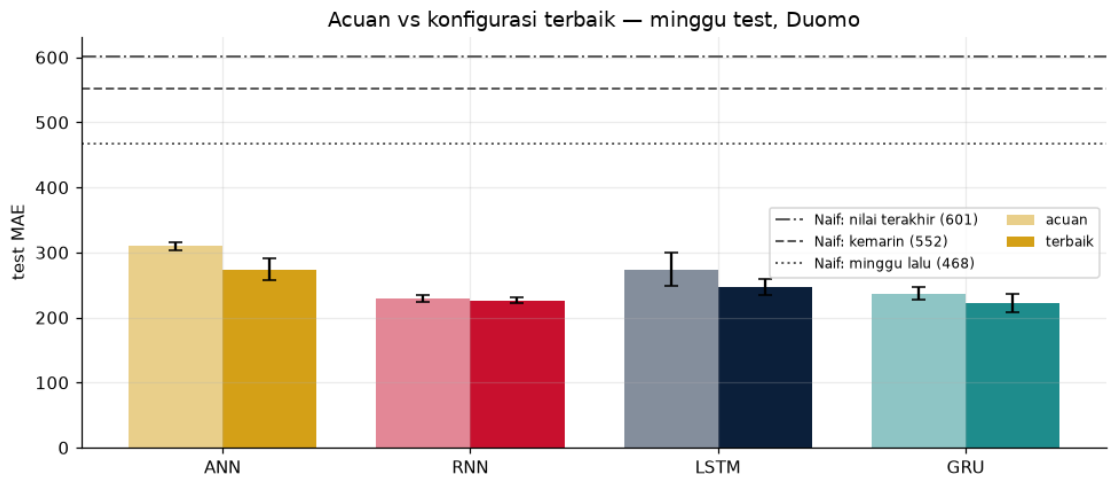
\includegraphics[width=\linewidth]{C_terbaik_vs_acuan.png}
  \caption{Test MAE konfigurasi acuan dan terbaik di Duomo. Garis horizontal: baseline naif (nilai terakhir, kemarin, minggu lalu).}
  \label{fig:terbaik}
\end{figure}
 
\subsection{Uji Generalisasi}
\label{sec:generalisasi}
Konfigurasi acuan dan terbaik dari Duomo dijalankan ulang tanpa diubah di Universita Bocconi (Tabel~\ref{tab:bocconi}).
 
\textbf{Urutan model berubah.} Pada acuan, RNN terbaik di Duomo (229,6) tetapi terburuk di Bocconi (754,2), sedangkan GRU terbaik di Bocconi (608,5). GRU tetap terbaik pada konfigurasi terbaik di kedua lokasi (552,3 di Bocconi). Namun std antar seed di Bocconi sangat besar (hingga $\pm 180{,}1$ pada LSTM), sehingga urutan ANN, GRU, dan LSTM pada acuan tidak pasti.
 
\textbf{Konfigurasi terbaik Duomo tidak selalu lebih baik.} Test MAE membaik pada RNN (turun 22,1\,\%), ANN (11,1\,\%), dan GRU (9,2\,\%), tetapi LSTM memburuk 27,8\,\% (682,1 $\to$ 871,8). Pada minggu Natal, konfigurasi terbaik hanya membantu RNN (1.100,3 $\to$ 789,3).
 
\textbf{Kaitan dengan pola trafik.} Gambar~\ref{fig:pola} menunjukkan trafik Bocconi turun bertahap sejak pertengahan Desember hingga sekitar 1.000 saat Natal (kemungkinan karena libur akhir tahun), padahal data latih berisi minggu-minggu sibuk dengan puncak sekitar 10.000. Model yang dilatih pada level tinggi meramal terlalu besar, sedangkan baseline nilai terakhir langsung mengikuti level terbaru. Akibatnya semua model kalah dari baseline tersebut (test 257,0; Natal 103,1), dengan MAPE 30--53\,\% dibanding 7--11\,\% di Duomo. MAPE GRU naik (31,1 $\to$ 41,8\,\%) walau MAE-nya turun, kemungkinan karena MAPE sangat dipengaruhi jam-jam sepi. Analoginya seperti belajar dari kalender kuliah yang sibuk lalu diuji saat libur panjang: model terbiasa pada keramaian, sedangkan baseline ``nilai terakhir'' cukup mengikuti kondisi sepi yang terbaru.
 
\begin{figure}[t]
  \centering
  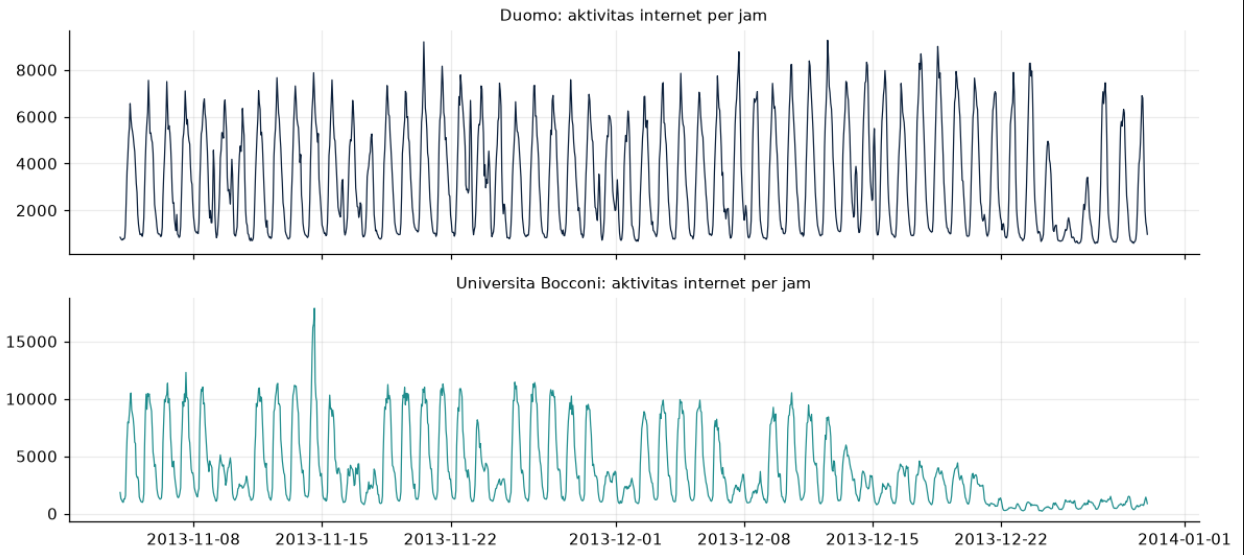
\includegraphics[width=\linewidth]{D_pola_lokasi.png}
  \caption{Aktivitas internet per jam di Duomo (atas) dan Universita Bocconi (bawah), November--Desember 2013.}
  \label{fig:pola}
\end{figure}
 
\begin{table}[t]
  \centering
  \caption{Hasil di Universita Bocconi (kode 2, kotak 4460), MAE kecuali dinyatakan lain}
  \label{tab:bocconi}
  \tabkecil
  \setlength{\tabcolsep}{1.8pt}
  \resizebox{\columnwidth}{!}{%
\begin{tabular}{@{}llcccc@{}}
    \toprule
    Model & Konf. & Val MAE & Test MAE & MAPE (\%) & Natal MAE \\
    \midrule
    \multicolumn{6}{@{}l}{\textit{Baseline naif (horizon 1 jam)}} \\
    Nilai terakhir & -- & 574,6 & \textbf{257,0} & -- & \textbf{103,1} \\
    Kemarin & -- & 1.093,4 & 611,1 & -- & 199,4 \\
    Minggu lalu & -- & 511,6 & 1.795,4 & -- & 1.405,1 \\
    \midrule
    \multicolumn{6}{@{}l}{\textit{Model}} \\
    ANN  & acuan   & $370{,}0 \pm 11{,}7$ & $645{,}5 \pm 57{,}0$ & $38{,}5 \pm 1{,}4$ & $817{,}3 \pm 240{,}2$ \\
         & terbaik & $338{,}5 \pm 23{,}3$ & $573{,}9 \pm 114{,}2$ & $31{,}7 \pm 9{,}4$ & $842{,}3 \pm 178{,}9$ \\
    RNN  & acuan   & $364{,}5 \pm 17{,}8$ & $754{,}2 \pm 85{,}7$ & $40{,}5 \pm 3{,}5$ & $1.100{,}3 \pm 180{,}9$ \\
         & terbaik & $314{,}0 \pm 11{,}0$ & $587{,}2 \pm 75{,}5$ & $30{,}3 \pm 4{,}3$ & $789{,}3 \pm 82{,}2$ \\
    LSTM & acuan   & $375{,}5 \pm 26{,}0$ & $682{,}1 \pm 180{,}1$ & $39{,}1 \pm 18{,}7$ & $1.240{,}3 \pm 409{,}1$ \\
         & terbaik & $311{,}4 \pm 10{,}8$ & $871{,}8 \pm 55{,}8$ & $52{,}8 \pm 8{,}5$ & $1.424{,}9 \pm 97{,}5$ \\
    GRU  & acuan   & $354{,}7 \pm 10{,}7$ & $608{,}5 \pm 127{,}4$ & $31{,}1 \pm 7{,}4$ & $836{,}9 \pm 206{,}2$ \\
         & terbaik & $308{,}4 \pm 3{,}6$ & $\mathbf{552{,}3 \pm 36{,}3}$ & $41{,}8 \pm 1{,}7$ & $933{,}5 \pm 113{,}2$ \\
    \bottomrule
  \end{tabular}}
\end{table}
 
% ---------------------------------------------------------------------
\section{Pembahasan}
\textbf{Faktor yang paling berpengaruh.} \textit{Learning rate} paling berpengaruh: test MAE GRU berubah dari 215,7 ($10^{-2}$) menjadi 356,3 ($10^{-4}$), selisih 140,6. Berikutnya jumlah lapisan untuk LSTM (273,6 $\to$ 412,6) serta panjang jendela dan \textit{dropout} untuk ANN (271,1 $\to$ 402,0 dan 309,9 $\to$ 411,6). Faktor yang hampir tidak berpengaruh adalah panjang jendela untuk RNN dan GRU, ukuran \textit{hidden} untuk ANN, \textit{batch size} 16 vs 64, dan jenis loss selain pada RNN. Penyebab utamanya sama: data latih hanya 672 sampel, jadi apa pun yang menambah kapasitas (jendela panjang pada ANN, lapisan tambahan) atau menambah gangguan (\textit{dropout} besar) lebih mudah merugikan daripada membantu. \textit{Learning rate} kecil merugikan karena 300 epoch tidak cukup untuk konvergen. Bayangkan belajar dari buku latihan yang hanya 4 minggu: tambahan beban lebih mudah membuat bingung daripada membantu.
 
\textbf{Model atau seed?} Perbedaan ANN dengan RNN dan GRU jelas lebih besar daripada perbedaan antar seed (selisih 73--80 vs std $\le 9{,}3$ pada acuan). Sebaliknya, RNN dan GRU tidak dapat dibedakan: selisih pada acuan 7,6 dan pada konfigurasi terbaik 4,4, keduanya lebih kecil daripada std GRU (9,3 dan 14,3). LSTM paling tidak stabil antar seed ($\pm 25{,}4$ pada acuan) dan tidak lebih baik daripada RNN sederhana. Penjelasan yang masuk akal: jendela hanya 24 jam, sehingga kelebihan LSTM dan GRU dalam mengingat informasi jauh belum diperlukan, sementara gerbangnya menambah parameter yang sulit dilatih dengan data kecil. Banyak selisih antar nilai \textit{hyperparameter} juga masih di dalam std (misalnya \textit{batch size} pada RNN), jadi kesimpulan dari 3 seed perlu hati-hati. Analoginya dua pelari yang selisih 0,1 detik, padahal waktu tiap pelari sendiri berubah 0,3 detik antar lomba; selisih sekecil itu belum bisa dipakai untuk menyatakan siapa yang lebih cepat.
 
\textbf{Val, test, dan Natal.} Memilih lewat val MAE tidak selalu menghasilkan test terbaik. RNN dengan loss MAE mencapai test 207,6 (terendah dari semua run Duomo yang kami laporkan), tetapi val MAE-nya lebih buruk daripada acuan, dan konfigurasi gabungan tidak lebih baik di val untuk tiga dari empat model. Val hanya satu minggu sehingga cukup berisik; val seperti ujian tryout dan test seperti ujian sungguhan, jadi nilai tryout satu minggu bisa kebetulan bagus atau buruk. Pada minggu Natal pola mingguan berubah karena libur, dan data latih tidak pernah memuat hari libur, sehingga sebagian besar model kalah dari baseline sederhana. Natal seperti soal bab yang belum pernah dipelajari.
 
\textbf{Keterbatasan.} (1) Hanya satu kota dan dua lokasi. (2) Data latih hanya 4 minggu (672 sampel), sehingga model berkapasitas besar sulit belajar. (3) Hanya satu kali pembagian waktu, sehingga satu minggu val dan test sangat menentukan hasil. (4) Hanya 3 seed, sehingga std yang dilaporkan kasar. (5) Faktor diubah satu per satu, jadi interaksi antar faktor tidak teramati.
 
% ---------------------------------------------------------------------
\section{Kesimpulan}
Di Duomo, model rekuren lebih baik daripada ANN: setelah penyetelan, GRU ($221{,}9 \pm 14{,}3$) dan RNN ($226{,}3 \pm 4{,}9$) terbaik, disusul LSTM ($246{,}6 \pm 12{,}0$) dan ANN ($273{,}9 \pm 17{,}0$), semuanya jauh di bawah baseline naif terbaik (467,6). Selisih GRU dan RNN lebih kecil daripada std, sehingga RNN yang ringan sudah cukup. \textit{Learning rate} paling berpengaruh, sedangkan jendela panjang pada ANN, lapisan tambahan, dan \textit{dropout} tinggi justru merugikan pada 672 sampel latih. Di Bocconi, GRU tetap terbaik ($552{,}3 \pm 36{,}3$), tetapi semua model kalah dari baseline nilai terakhir (257,0) karena pola trafik berubah menjelang Natal, sehingga model perlu diuji ulang di tiap lokasi.
 
% ---------------------------------------------------------------------
\section*{Kontribusi Anggota}
\begin{tabular}{@{}lp{0.55\linewidth}@{}}
  Alfita Eryani Nugroho: Running all code, penulisan hasil\\
  Octavia Sesilia Malau: Penyusunan laporan\\
  Fitria Oktavianti: Penyusunan laporan
\end{tabular}
 
\section*{Pernyataan Penggunaan AI}
Claude (Anthropic) dipakai untuk membantu menyusun draf teks dan merapikan bahasa laporan berdasarkan hasil run kelompok. Seluruh angka berasal dari run kami sendiri.
 
\section*{Kode dan Data}
Kode, notebook beserta output, dan seluruh hasil run tersedia di \url{https://github.com/ALF-002/Tugas-AI-RB-Fita}.
 
\bibliographystyle{IEEEtran}
\bibliography{references}
 
\end{document}
 